\documentclass[10pt, a4paper]{scrartcl}

\usepackage{qrcode}

\usepackage{vorschule}
\usepackage[
    typ=ab,
    fach=Informatik,
    lerngruppe={9Diff},
    nummer=3,
    module={Symbole,Lizenzen},
    seitenzahlen=keine,
    farbig,
    lizenz=cc-by-nc-sa-4,
]{schule}

\usepackage[
	kuerzel=Ngb,
	reihe={Der KnowHowPC},
	version={2019-10-07},
]{ngbschule}

\author{J. Neugebauer}
\title{Wie arbeitet ein Computer?}
\date{\Heute}

\setzeAufgabentemplate{ngbnormal}


\begin{document}

\ReiheTitel

\begin{aufgabe}[symbol=\symLaptop]
	Im Tauschordner findest du ein weiteres Programm für den \emph{KnowHowPC}: \ordner{Drittes Programm.khp}.
	
	\begin{center}
		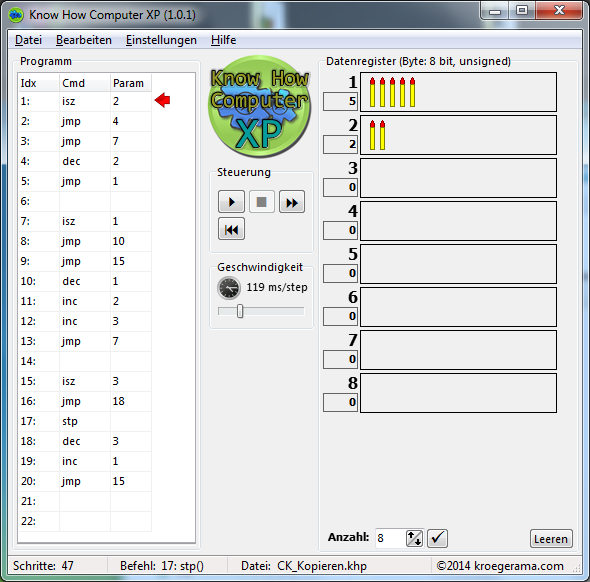
\includegraphics[width=0.8\textwidth]{9Diff-AB.3-Abb-1}
	\end{center}
	
	\begin{teilaufgaben}
		\teilaufgabe Gib nun in das Register 1 fünf Streichhölzer ein und in das Register 2 zwei. Lass das Programm im \emph{Einzelschritt-Modus} ablaufen.
		
		\teilaufgabe Probiere andere Kombinationen an Werte in den Registern aus – auch welche, in der Register 1 oder 2 leer sind.
		
		\teilaufgabe Beschreibe, was das Programm leistet.
		
		\teilaufgabe Zeichne für das Programm ein \emph{Ablaufdiagramm}.
		
		\teilaufgabe Erläutere nun, wie das Programm seine Aufgabe erledigt.
		
		\emph{Beachte:} Das Programm besteht aus drei Blöcken: Zeile 1-5, Zeile 7-13 und Zeile 15-20. Jeder Block ist für eine andere Teilaufgabe zuständig.
		
		\teilaufgabe\label{ta:impl1} Verändere das Programm so, das die Bedeutung von Register 1 und 2 vertauscht ist.
		
		\teilaufgabe\symStern\ Verändere das Programm aus \ref{ta:impl1} so, dass nach Beendigung des Programms Register 1 immer doppelt so viele Hölzer enthält, wie Register 2.
	\end{teilaufgaben}
\end{aufgabe}


\end{document}
